\def\QRCODE{TB_IPR_TUT.IMG.hough_pythonqrcode.png}
\def\QRPAGE{http://www.iptutorials.science/tree/master/TB_IPR/TUT.IMG.hough/python}
\pcorrectionsection{Python correction}

This correction makes use of the python modules numpy, opencv, skimage and matplotlib.
\begin{python}
import numpy as np
import cv2
import matplotlib.pyplot as plt
from skimage.feature import peak_local_max
\end{python}

\subsection{Contours detection}
The contours are detected using the Canny edge detection method. In this code, the method from OpenCV is employed, see Fig.\ref{fig:hough:python:canny}.

\begin{python}
img = cv2.imread('TestPR46.png');
plt.figure()
plt.imshow(img)

# perform contours detection
edges = cv2.Canny(img,100,200);
plt.figure()
plt.imshow(edges)
\end{python}

\begin{figure}[htbp]
 \centering
 \subfloat[Canny edge detection.]{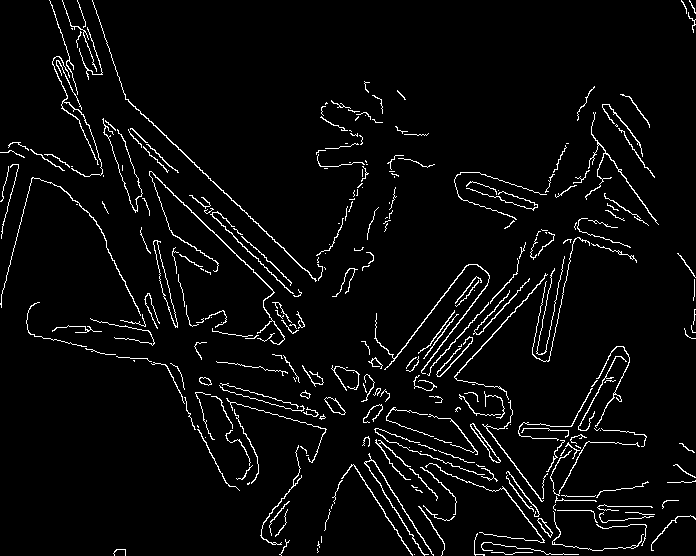
\includegraphics[width=.45\linewidth]{edges_hough.python.png}\label{fig:hough:python:canny}}\hfill 
 \subfloat[Representation of the sinogram and detection of the maxima in the Hough space.]{ 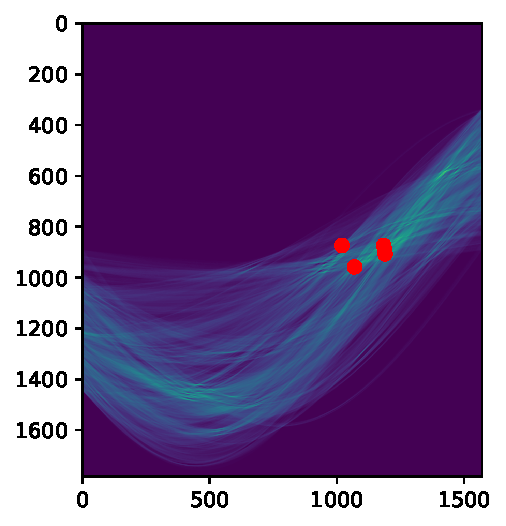
\includegraphics[width=.45\linewidth]{sinogram_hough.python.pdf}\label{fig:hough:python:sinogram}}
 
 \caption{The algorithm of the Hough line detection consists in detecting the edges, then representing each pixel in the Hough space and finally detecting the maximal value in the sinogram.}
 \label{fig:hough:python:algo}
\end{figure}


\subsection{Hough transform}
Notice that OpenCV contains Hough fonctions: \pinline{HoughLines} and \pinline{HoughLinesP}. The result (sinogram) of the image is presented Fig.\ref{fig:hough:python:sinogram}.


\begin{python}
## Hough transform
# size of image
X = img.shape[0];
Y = img.shape[1];

angular_sampling = 0.01; # angles in radians

# initialization of matrix H
rho_max = np.hypot(X,Y);
rho = np.arange(-rho_max, rho_max, 1);
theta = np.arange(0, np.pi, angular_sampling);
cosTheta = np.cos(theta);
sinTheta = np.sin(theta);
H = np.zeros([rho.size, theta.size]);

# Hough transform
# loop on all contour pixels
for i in range(X):
    for j in range(Y):
        if (edges[i,j] != 0):
            R = i*cosTheta + j*sinTheta;
            R = np.round(R + rho.size/2).astype(int);
            H[R,range(theta.size)] += 1;

plt.imshow(H);
\end{python}

\subsection{Maxima detection}
The function \pinline{peak_local_max} from \pinline{skimage} is used to detect local maxima in the Hough transform. Matrix H is first smoothed with a Gaussian filter and represented in Fig.\ref{fig:hough:python:sinogram}.
\begin{python}
# Maxima detection
G = cv2.GaussianBlur(H, (5,5), 5);
maxima = peak_local_max(H, 5, threshold_abs=150, num_peaks=5);
plt.figure();
plt.imshow(G);

# display maxima on Hough transform image G
plt.scatter(maxima[:,1], maxima[:,0], c='r');
plt.show();
\end{python}

\subsection{Resulting lines}
The result is shown in Fig.\ref{fig:hough:python:hough}.
\begin{python}
# display the results as lines in image
for i_rho, i_theta in maxima:
    print rho[i_rho], theta[i_theta]
    a = np.cos(theta[i_theta])
    b = np.sin(theta[i_theta])
    y0 = a*rho[i_rho]
    x0 = b*rho[i_rho]
    y1 = int(y0 + 1000*(-b))
    x1 = int(x0 + 1000*(a))
    y2 = int(y0 - 1000*(-b))
    x2 = int(x0 - 1000*(a))
    
    cv2.line(img,(x1,y1),(x2,y2),(0,0,255),2)

# display in window
cv2.imshow('hough transform', img);
# write resulting image
cv2.imwrite('cv_hough.png', img);
\end{python}

\begin{figure}
 \centering
 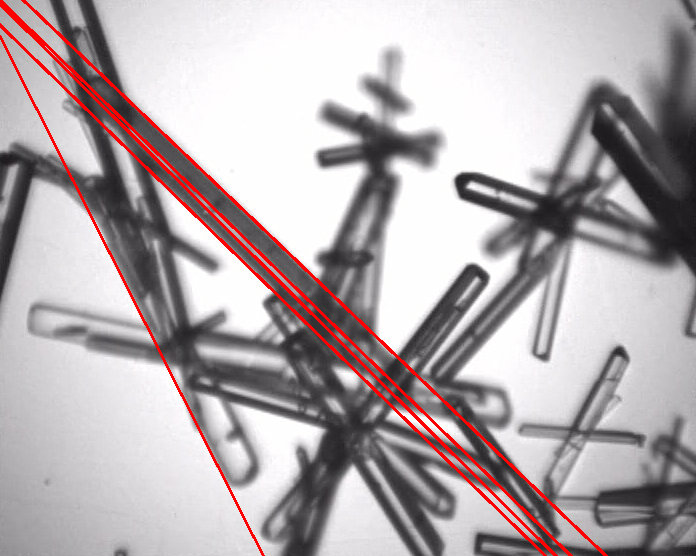
\includegraphics[width=10cm]{cv_hough.png}
 \caption{Lines detected with the Hough transform.}
 \label{fig:hough:python:hough}
\end{figure}


\subsection{OpenCV builtin function}
\begin{python}
import cv2
import numpy as np

# read image and convert it to gray
img = cv2.imread('TestPR46.png')
gray = cv2.cvtColor(img,cv2.COLOR_BGR2GRAY)
edges = cv2.Canny(gray, 100, 200, apertureSize = 3)

# threshold value for lines selection:
# lower value means more lines
threshold = 150;

# perform lines detection
lines = cv2.HoughLines(edges, 1, np.pi/180, threshold)

# display lines
for rho,theta in lines[0]:
    print rho, theta
    a = np.cos(theta)
    b = np.sin(theta)
    x0 = a*rho
    y0 = b*rho
    x1 = int(x0 + 1000*(-b))
    y1 = int(y0 + 1000*(a))
    x2 = int(x0 - 1000*(-b))
    y2 = int(y0 - 1000*(a))
    print x1, y1, x2, y2
    cv2.line(img,(x1,y1),(x2,y2),(0,0,255),2)

cv2.imshow('hough transform', img);
cv2.imwrite('cv_hough.png', img);
\end{python}
